\section{Chapitre 1 - S�rie de Taylor}

\setcounter{cor}{0}
\begin{cor}[Polyn�me de Taylor]
\begin{enumerate}
	\item $T_{3,0}(x) = 1 + x + \dfrac{x^2}{2} + \dfrac{x^3}{6}$
	\item \begin{align*}
				f(x)&=e^x  		&f(0)&=\textcolor{red}{1} 		&T_{3,0}(x) &= 1 + x + \dfrac{x^2}{2} + \dfrac{x^3}{6}		&T_{3,0}(0)&=\textcolor{red}{1} \\
				f'(x)&=e^x  		&f'(0)&=\textcolor{red}{1} 		&T_{3,0}'(x) &= 1 + x + \dfrac{x^2}{2}		&T_{3,0}'(0)&=\textcolor{red}{1} \\
				f''(x)&=e^x  		&f''(0)&=\textcolor{red}{1} 		&T_{3,0}''(x) &= 1 + x 		&T_{3,0}''(0)&=\textcolor{red}{1} \\
				f^{(3)}(x)&=e^x  		&f^{(3)}(0)&=\textcolor{red}{1} 		&T_{3,0}^{(3)}(x) &= 1 		&T_{3,0}^{(3)}(0)&=\textcolor{red}{1} \\
				\end{align*}
\end{enumerate}
\end{cor}

\medskip

\begin{cor}[Polyn�me de Taylor suite ...]
\begin{enumerate}
	\item On a $T_{3,0}(x) = 1 + x + \dfrac{x^2}{2} + \dfrac{x^3}{6}$, donc une bonne approximation de $e^{0,1}$ peut �tre donn�e par
				\begin{align*}
				T_{3,0}(0,1)
				&= 1 + 0,1 + \dfrac{0,1^2}{2} + \dfrac{0,1^3}{6} \\
				&= 1,1 + \dfrac{0,01}{2} + \dfrac{0,001}{6} \\
				&= \dfrac{6,631}{6}\\
				&\approx 1,105~166~666...
				\end{align*}
	\item D'apr�s la formule de Taylor-Lagrange, l'erreur commise est major�e par $\left|\dfrac{(x-a)^{n+1}}{(n+1)!} f^{(n+1)}(c)\right|$ avec $c\in]a;x[$, $a=0$, $x=0,1$ et $n+1=4$. Autrement dit
$$\left|\dfrac{0,1^{4}}{4!} f^{(4)}(c)\right| \quad \text{ avec  }c\in]0;0,1[$$
				$f^{(4)}(x)=e^x$, une fonction positive et croissante. Sur $]0;0,1[$ elle est major�e par $e^{0,1}$... Probl�me c'est la valeur que je cherche � approximer. Par contre, $0,1<\ln 2$ donc je peux majorer par $e^{\ln 2} = 2$.\\
				L'erreur commise est donc major�e par
				$$\left|\dfrac{0,1^{4}}{4!} f^{(4)}(c)\right| \leq \dfrac{0,1^4}{4\times 3\times 2\times 1} \times 2 = \dfrac{0,000~1}{12} \approx 0,000~008~333...$$
				\textcolor{red}{Si je veux un compte juste, je peux prendre $0,1<\ln 3$ donc je peux majorer par $e^{\ln 3} = 3$.\\
				L'erreur commise est donc major�e par
				$$\left|\dfrac{0,1^{4}}{4!} f^{(4)}(c)\right| \leq \dfrac{0,1^4}{4\times 3\times 2\times 1} \times 3 = \dfrac{0,000~1}{8} = 0,000~012~5$$}
				La calculatrice donne $e^{0,1} \approx 1,105~170~918...$. Trois d�cimales exactes.
	\item En prenant b�tement notre polyn�me de Taylor au voisinage de 0 :
				\begin{align*}
				T_{3,0}(1)
				&= 1 + 1 + \dfrac{1^2}{2} + \dfrac{1^3}{6} \\
				&= 2 + \dfrac{1}{2} + \dfrac{1}{6} \\
				&= \dfrac{12 + 3 + 1}{6} \\
				&= \dfrac{16}{6}\\
				&= \dfrac{8}{3}\\
				&\approx 2,666~666...
				\end{align*}		
				Or : $e^{1} \approx 2,718~281~82...$. L'erreur commise est assez importante. En effet, elle est major�e par :
				$$\left|\dfrac{1^{4}}{4!} f^{(4)}(c)\right| \leq \dfrac{1^4}{4\times 3\times 2\times 1} \times e^{1} = \dfrac{e}{24} \approx 0,113~261...$$
				ce qui n'est plus du tout n�gligeable.
\end{enumerate}
\end{cor}

\begin{cor}[... et fin]
\begin{enumerate}
	\item $f(x)=\dfrac{1}{1-x}$
				\begin{align*}
				f(x)&=\dfrac{1}{1-x}, &f'(x)&=\dfrac{1}{(1-x)^2}, &f''(x)&=\dfrac{2}{(1-x)^3}, &f^{(3)}(x) &= \dfrac{6}{(1-x)^4}, &f^{(4)}(x)&=\dfrac{24}{(1-x)^5}, &f^{(5)}(x)&=\dfrac{60}{(1-x)^6} \\
				f(0)&=1, &f'(0)&=1, &f''(0)&=2, &f^{(3)}(0) &= 6, &f^{(4)}(0)&=24 &&
				\end{align*}
				D'apr�s la formule de Taylor-Lagrange :
				$$f(x)=\dfrac{1}{1-x} = 1 + x + x^2 + x^3 + x^4 + \dfrac{x^5}{(1-c)^6}, \qquad \text{avec } c\in]0,x[$$
	\item $g(x)=\ln(1+x)$
				\begin{align*}
				g(x)&=\ln(1+x), &g'(x)&=\dfrac{1}{1+x}, &g''(x)&=-\dfrac{1}{(1+x)^2}, &g^{(3)}(x) &= \dfrac{2}{(1+x)^3}, &g^{(4)}(x)&=-\dfrac{6}{(1+x)^4}, &g^{(5)}(x)&=\dfrac{24}{(1+x)^5} \\
				g(0)&=0, &g'(0)&=1, &g''(0)&=-1, &g^{(3)}(0) &= 2, &g^{(4)}(0)&=-6 &&
				\end{align*}
				D'apr�s la formule de Taylor-Lagrange :
				$$g(x)=\ln(1+x) = x - \dfrac{x^2}{2} + \dfrac{x^3}{3} - \dfrac{x^4}{4} + \dfrac{x^5}{5(1+c)^5}, \qquad \text{avec } c\in]0,x[$$
	\item $h(x)=\sin(2x)$
				\begin{align*}
				h(x)&=\sin(2x), &h'(x)&=2\cos(2x), &h''(x)&=-4\sin(2x), &h^{(3)}(x) &= -8\cos(2x), &h^{(4)}(x)&=16\sin(2x), &h^{(5)}(x)&=32\cos(2x) \\
				h(0)&=0, &h'(0)&=2, &h''(0)&=0, &h^{(3)}(0) &= -8, &g^{(4)}(0)&=0 &&
				\end{align*}
				D'apr�s la formule de Taylor-Lagrange :
				$$h(x)=\sin(2x) = 2x - \dfrac{4}{3}x^3 + \dfrac{8}{15}x^5\cos(2c), \qquad \text{avec } c\in]0,x[$$
\end{enumerate}
\end{cor}


\begin{cor}[Scilab]
\lstinputlisting[language=Scilab]{01-Serie-de-Taylor/Scripts-Scilab/ex4-erreur.sci}
Le r�sultat est alors $n=10$. En effet on a alors $\dfrac{0,1^n}{n!} \approx 2,7557319223985907\times 10^{-17}.$\\
L'erreur de calcul commise est alors inf�rieure � la pr�cision de calcul de Scilab.
\end{cor}



\begin{cor}[Polyn�me de Taylor avec Scilab]
Avec le code suivant :
\lstinputlisting[language=Scilab]{01-Serie-de-Taylor/Scripts-Scilab/ex5-exponentielle.sci}
On obtient les r�sultats suivants :\\
\begin{tabularx}{\textwidth}{XX}
\begin{center}
	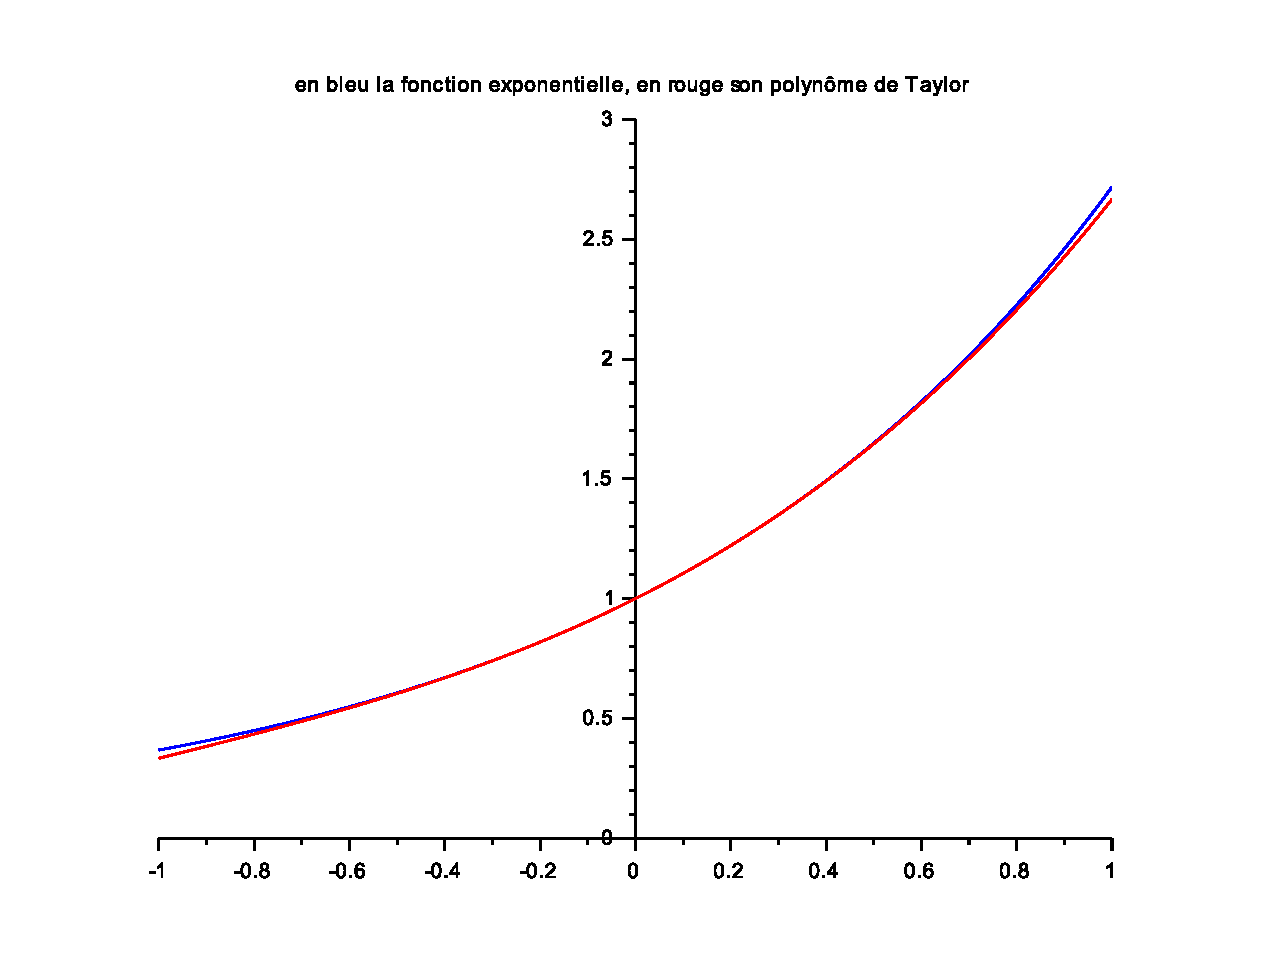
\includegraphics[width=0.45\textwidth]{01-Serie-de-Taylor/Scripts-Scilab/ex5-1.pdf}\newline
	Pour \textbf{graphes(-1,1)}
\end{center}
&
\begin{center}
	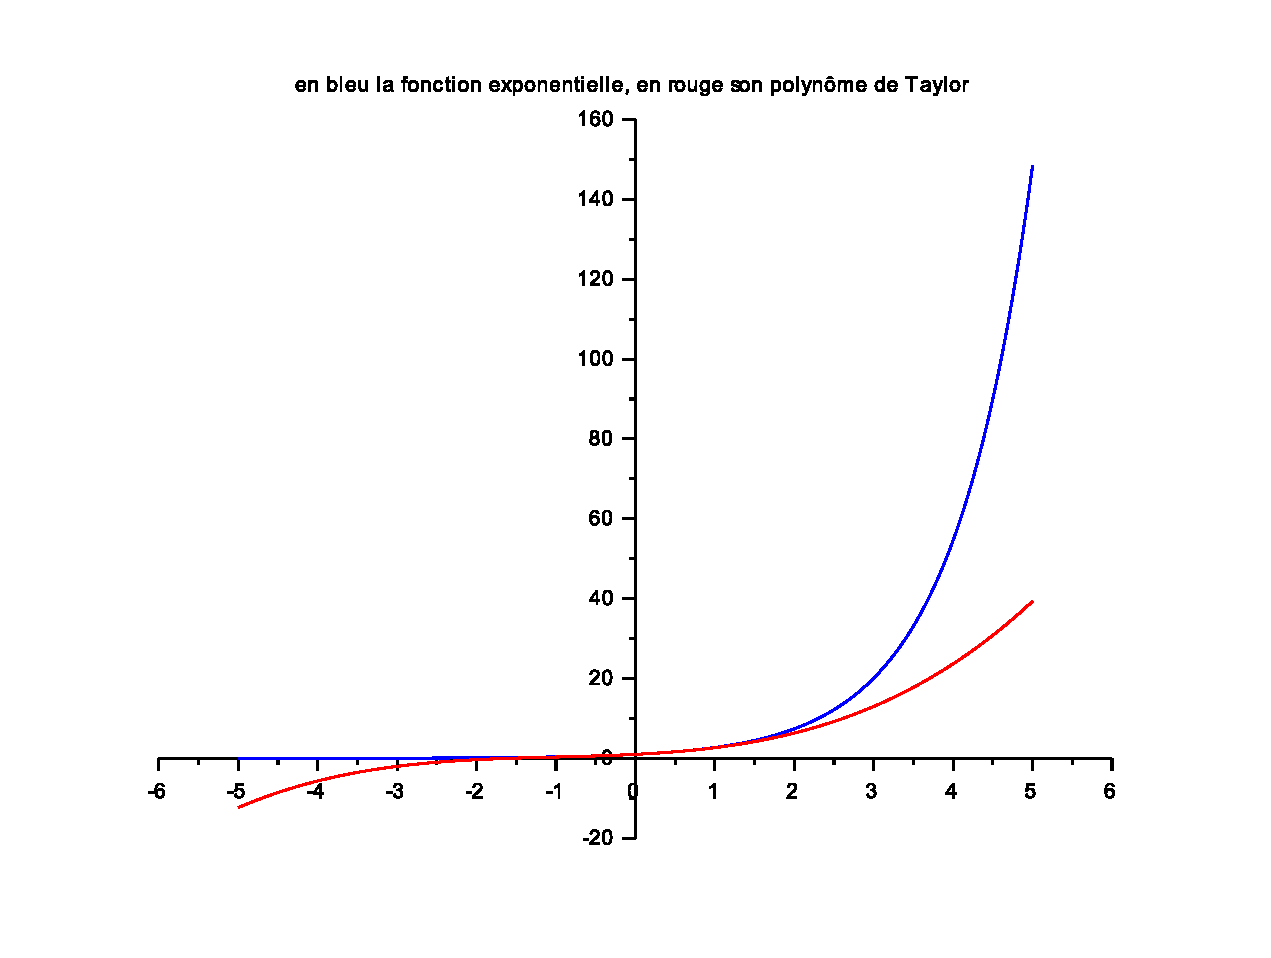
\includegraphics[width=0.45\textwidth]{01-Serie-de-Taylor/Scripts-Scilab/ex5-5.pdf}\newline
	Pour \textbf{graphes(-5,5)}
\end{center}
\end{tabularx}
\end{cor}
